This path-sensitive reachability-bound algorithm
is performed on basis of an \emph{Abstract Transition Graph} for the program $c$.
This step shows how to generate the abstract transition graph $\absG(c)$ of a
program $c$ through constructing its vertices and edges.

\subsection{Vertices}
\label{sec:abs_prog-vertex}
Every 
vertex corresponds to a program execution point, 
and the vertices set is all the $c$'s program execution points with an extra exit point ${\lex}$, 
\[ 
  \absV(c) = \lvar(c)\cup\{{\lex}\}
  \]

\subsection{Edges}
\label{sec:abs_prog-edge}
  In the first step, \textbf{Constraint Computation} generates the constraint
  for the expression in each program command,
  which is used as the annotation of an edge.
  \\
The second step, generates two sets for each command, which are \textbf{Initial and Continuation Execution Program Points}. 
  The initial set contains the
  program point where this command {starts} to execute, 
  and the continuation set contains both the constraint of this command
  and the continuation program points after the execution of this command.
  \\ 
  In the third step, \textbf{Abstract Event Computation} generates a set of edges for the program.
  Each edge is a pair of initial and finial state.
%
\paragraph{Constraint Computation}
In this step, we first show how to compute the constraints for expressions in a program $c$,
by a program abstraction method adopted from the
algorithm in Section 6 in~\cite{SinnZV17}.
\\
Given a program $c$,
every arithmetic expression in an assignment command with label $l$,
or boolean expression in the guard of a $\eif$ or $\ewhile$ command with label $l$
is transformed into a constraint.
\\
This constraint describes the abstract execution of the assignment command with label $l$,
or abstract evaluation of the boolean expression in the guard with label $l$.

\highlight{Notations / Formal Definitions:}
\begin{itemize}
\item Operator: $\absexpr : \mathcal{A} \cup \booldom \to DC(\vardom  \cup \scvardom)\cup \booldom \cup \{\top\}$
%
\item Constraints $\dcdom^{\top}: DC(\vardom  \cup \scvardom) \cup \booldom\cup \{\top\}$  contains:
%
\begin{itemize}
\item The difference constraints $DC(\vardom  \cup \scvardom)$ is the set of all the inequality of
form $x' \leq y + v$ or $x' \leq v$ where $x \in \vardom $, 
$y \in \vardom$ and $v \in \scvardom$.
\\
The \emph{Symbolic Constant} can be a natural number, $\infty$, or a program's input variable, We use $\scvardom \subseteq \mathbb{N} \cup \vardom \cup \{\infty \}$ to denote the universe of all \emph{Symbolic Constant},
which is the set of all natural numbers with $\infty$ and programs' input variables.
\\
An inequality $x' \leq y + v$ describes that the value of $x$ in the current state is
at most the value of $y$ in the previous state plus the symbolic constant $v$.
An inequality $x' \leq v$ describes that the value of $x$ in the current state is
at most the value $v$.
When a difference constrain shows up as an edge annotation, $l \xrightarrow{x' \leq y + v} l'$,
% Then $x'$ 
it denotes that
the value of variable $x$
after executing the command at $l$ is at most
% and the right-hand side describes 
the value of variable $y$ plus $v$ before the execution,
and $l \xrightarrow{x' \leq v} l'$ respectively denotes value of variable $x$
after executing the command at $l$ is at most
% and the right-hand side describes 
the value of the symbolic constant $v$ before the execution.
For every expression in each of the label command, it is computed in three steps via program abstraction method adopted from the Section~6 in~\cite{SinnZV17}. 
%
\item The Boolean Expressions $b$ from the set $\booldom$.
$b$ on an edge $l \xrightarrow{b} l'$ describes
that after evaluating the guard with label $l$,
$b$ holds and the command with label $l$ will execute right after.
%
\item The top constraint, $\top$ denotes true. It is preserved for $\eskip$ command,
or commands that don't interfere any guard variable.
\end{itemize}
\end{itemize}

\highlight{Computation Steps:}

\begin{defn}[Symbolic Expression of a Program($\scexpr(c)$)]
  \label{def:symbolic_expr}
  $\scexpr(c)$ is the set of all the arithmetic expressions over $\mathbb{N} \cup \inpvar(c) \cup \{\infty \}$ for a given program $c$.
\end{defn}

\begin{defn}[Constraint Computation]
  \label{def:constraint_compute}
  For a program $c$, a boolean expression $\bexpr$ in the guard of a $\eif$ or $\ewhile$ command
  or an expression $\expr$ and a variable $x$
  in an assignment command $\assign{x}{\expr}$,
  the constraint $\absexpr(\bexpr, \_, c )$ or $\absexpr(x - v, x, c)$ is computed as follows.
  \begin{enumerate}
  \item Compute the symbolic constant set of program $c$, $\scvar(c)$ of program $c$ as follows.
  \[
    \scvar(c) = \mathbb{N} \cup \inpvar(c) \cup \{\infty \} \subseteq \scvardom
  \]
  \item Initialize 
  $\grdvar(c) = \{\}$ as the set of the variable used in the expression of every while or if guard in the program $c$.
  \item Then we compute  $\absexpr(\bexpr, \_, c )$ or $\absexpr(x - v, x, c)$.
  \[
    \begin{array}{ll} 
      \absexpr(x - v, x, c)  = x' \leq x - v  & x \in \grdvar(c)\land v \in \scvar(c) \\
      \absexpr(y + v, x, c)  = x' \leq y + v  & x, y \in \grdvar(c)\land v \in \scvar(c)\\
      \absexpr(v, x, c)  = x' \leq v  & x \in \grdvar(c)\land v \in \scvar(c) \\
      \absexpr(y + v, x, c)  = x' \leq y + v, \grdvar(c) = \grdvar(c) \cup \{y\} 
      & x \in \grdvar(c)\land y \notin \grdvar(c) \land v \in \scvar(c)  \\
      \absexpr(\bexpr, \_, c) = \bexpr, \grdvar(c) = \grdvar(c) \cup FV(\bexpr) & \bexpr \in \scvar(c) \\
      \absexpr(\expr, x, c) = \top &  {o.w.} \\
    \end{array}
    \]
  \end{enumerate}
   $\absexpr(\expr, x, c)$ and $\grdvar(c)$ are iteratively updating until stabilized over every guard and assignment command in $c$. In the following part of the paper, we use $\absexpr(\expr, x, c)$
   to denote the stabilized computation result.
  \end{defn}
%
In the case 4, if a variable $x$, belonging to the set 
  $\grdvar(c)$ is updated by a variable $y$, which isn't in this set, 
  we add $y$ into the set $\grdvar(c)$ and repeat 
  above procedure  until $\grdvar(c)$ and $\absexpr(\expr, x, c)$ is stabilized. 
  \\
Specifically 
we handle a 
normalized expression, $x > 0$
in guards of if and while loop headers, and 
the guard variable $x$ only increase, decrease or reset by 
simple arithmetic expression (mainly multiplication, division, minus and plus (able to extend to max and min)). 
The guard variable $x$ is generalized into the \emph{norm} when the guard 
in if or while has the form $\expr > 0$ with an expression $\expr$, and $\grdvar$ is the set of norms.
Then in the last clause in Definition~\ref{def:constraint_compute}, i.e., $\absexpr(\expr, x, c)$,
we will check if $\expr$ is a norm or contains norms, and extend the $\grdvar(c)= \grdvar(c)\cup \{\expr\}$ if neither.
The constraint computation over the \emph{norm} follows the computation steps 1, 2 and 3 in Section 6.1 in paper~\cite{SinnZV17}. 
%
\paragraph{Abstract Initial and Continuation State Computation}
This step computes two sets for each command. 
The initial state is a set that contains the
program points before executing this command, which is computed by the standard initial state generation method from control flow analysis.
The final state is a set
that contains the constraint of this command and the program points after the execution of this command.
This set is enriched 
from the standard control flow analysis.

%
\begin{itemize}
  \item The \emph{initial execution point}, $\absinit(c) \in \ldom$
  for a command $c$.
  $\absinit(c)$ is a unique program label corresponds to the command before executing this command. 
\\
Given a program $c$, its abstract initial state, $\absinit(c)$ is computed as follows,
%
\[
  \begin{array}{ll}
    \absinit(\clabel{\assign{x}{\expr}}{}^l)  & = l  \\
    \absinit(\clabel{\eskip}^{l})  & = l \\
    \absinit(\eif (\clabel{\bexpr}^l, c_t, c_f))  & = l \\
    \absinit(\ewhile \clabel{\bexpr}^l \edo (c_w))  & = l \\
    \absinit(c_1 ; c_2)  & = \absinit(c_1) \\
 \end{array}
 \]
%
%
\item The \emph{continuation execution state}, $\absfinal(c)$ of program $c$, 
$\absfinal(c) \in \mathcal{P}(\ldom \times \dcdom^{\top})$
is a set of pairs, $(l, dc)$ with a
program point (i.e., a label), $l$ as the first component and a constraint, 
$dc$ as the second component.
The program point $l$ corresponds to the labeled command after the execution of $c$,
and the constraint $dc$ in this pair is computed by $\absexpr$ for the expression in $c$.
%  in the first step.
\\
Given a program $c$, its final state, $\absfinal(c)$ is computed as follows,
 \[
  \begin{array}{ll}
    \absfinal(\clabel{\assign{x}{\expr}}{}^l)  & = \{(l, \absexpr(\expr, x, c))\}  \\
     \absfinal(\clabel{\eskip}^{l})  
     & = \{(l, \top)\} \\
     \absfinal(\eif (\clabel{\bexpr}^l, c_t, c_f))  & = \absfinal(c_t) \cup \absfinal(c_f) \\
     \absfinal(\ewhile \clabel{\bexpr}^l \edo (c_w))  & = \{(l, \absexpr(\bexpr, \top, c_w))\} \\
     \absfinal(c_1 ; c_2)  & =  \absfinal(c_2) \\
 \end{array}
 \]
 %
\end{itemize}
 \paragraph{Abstract Event Computation} Each abstract event is an edge between two vertices in the abstract transition graph.
 It is generated by computing the initial and continuation execution state interactively and recursively for a program $c$.
 
 \highlight{Notations and Formal Definitions:}
 \begin{itemize}
  \item \emph{Abstract Event}: 
  $\absevent \in $
  $\ldom \times \dcdom^{\top} \times \ldom$
  \item \emph{Abstract Trace}, $\absflow(c)$ of a program $c$: $\absflow(c) \in \mathcal{P}( \ldom \times \dcdom^{\top} \times \ldom )$
 \end{itemize}
 \begin{defn}[Abstract Event]
   \label{def:abs_event}
   Abstract Event: 
   $\absevent \in $
   $\ldom \times \dcdom^{\top} \times \ldom$
   is a 
   triple where the first and third components are labels,
   second component is a constraint from $\dcdom^{\top}$.
   \end{defn}
   In an abstract event $(l, dc, l')$ of a program $c$, 
   the first label $l \in \ldom$ corresponds to the \emph{initial execution point} $\absinit(c)$ of $c$, and 
   the second label $l' \in \ldom$ with the constraint $dc \in \dcdom^{\top}$ correspond to an abstract continuation execution state of $c$.
We abuse the notation $\mathcal{P}(\absevent)$ for the power set of all abstract events.

\highlight{Computation Steps:}
\\
The set of the abstract events $\absflow(c)$ for a program $c$
is computed as follows in Definition~\ref{def:absevent_compute}.
 %
 \begin{defn}[Abstract Trace Computation]
 \label{def:absevent_compute}
 The \emph{abstract trace}, $\absflow(c) \in \mathcal{P}( \ldom \times \dcdom^{\top} \times \ldom )$ of a program $c$  is computed as follows.

 We first append a $\eskip$ command with 
the label $\lex$, i.e., $\clabel{\eskip}^{{\lex}}$ at the end of the program $c$, and construct 
the program $c' = c;\clabel{\eskip}^{{\lex}}$.
Then, we compute the $\absflow(c) = \absflow'(c')$ for $c'$ as follows,
 %
 {
 \[
   \begin{array}{ll}
      \absflow'(\clabel{\assign{x}{\expr}}{}^l)  & = \emptyset  \\
      \absflow'([\eskip]^{l})  & = \emptyset \\
      \absflow'(\eif (\clabel{\bexpr}^l, c_t, c_f))  & =  \absflow'(c_t) \cup \absflow'(c_f)
        \\ & \quad 
        \cup \{(l, \absexpr(\bexpr, \top, c),  \absinit(c_t) ) ,  (l, \absexpr(\neg\bexpr, \top, c), \absinit(c_f)) \} \\
       \absflow'(\ewhile \clabel{\bexpr}^l \edo (c_w))  & =  \absflow'(c_w) \cup \{(l, \absexpr(\bexpr, \top, c), \absinit(c_w)) \} 
       \\ & \quad 
       \cup \{(l', dc, l)| (l', dc) \in \absfinal(c_w) \} \\
       \absflow'(c_1 ; c_2)  & = \absflow'(c_1) \cup  \absflow'(c_2) 
       \\ & \quad 
       \cup \{ (l, dc, \absinit(c_2)) | (l, dc) \in \absfinal(c_1) \} \\
   \end{array}
   \]
   }
  \end{defn}
  Notice $\absflow'([x := \expr]^{l})$ and $\absflow'([\eskip]^{l})$ are both empty set. 
   For every event $\event$ with label $l$ in an execution trace $\trace$ of program $c$, 
   there is an abstract event in program's abstract execution trace of form $(l, \_, \_)$.  
   We also show the soundness of the \emph{abstract event computation} as Theorem~\ref{lem:abscfg_sound} below with proof in Appendix~\ref{apdx:abs_sound}.
\begin{lem}[Soundness of the Abstract Trace Computation]
\label{lem:abscfg_sound}
For every program $c$ and
a finite execution trace $\trace \in \ftdom$ which is generated w.r.t.
an initial trace  $\trace_0 \in \ftdom_0(c)$,
there is an abstract event $\absevent = (l, \_, \_) \in \absflow(c)$ 
for every event $\event \in \trace$ having the same label $l$, i.e., $\event = (\_, l, \_)$.
%
\[
\begin{array}{l}
  \forall c \in \cdom, \trace_0 \in \ftdom_0(c), \trace \in \ftdom ,  \event = (\_, l, \_) \in \eventset \st
  \big(
    \config{{c}, \trace_0} \to^{*} \config{c', \trace_0 \tracecat \trace} 
  % \lor 
  % \config{{c}, \trace_0} \uparrow^{\infty} \trace_0 \tracecat \trace 
  \big)
  \land \event \in \trace 
  \\
  \qquad \implies \exists \absevent = (l, \_, \_) \in (\ldom\times \dcdom^{\top} \times \ldom) \st 
  \absevent \in \absflow(c)
\end{array}
\]
\end{lem}
If $l$ is the label of an assignment command in a program $c$,
then there is a unique abstract event in the program's abstract events set
$\absevent \in \absflow(c)$ of form $(l, \_, \_)$. This uniqueness property is formally below as Lemma~\ref{lem:abscfg_unique} below
and proved in Appendix~\ref{apdx:abs_sound}.
\begin{lem}[Uniqueness of the Abstract Events]
\label{lem:abscfg_unique}
For every program $c$ and
a finite execution trace $\trace \in \ftdom$ which is generated w.r.t.
an initial trace $\trace_0 \in \ftdom_0(c)$,
there is a unique abstract event $\absevent = (l, \_, \_) \in \absflow(c)$ 
for every assignment event $\event \in \eventset^{\asn}$ in the
execution trace having the label $l$, i.e., $\event = (\_, l, \_)$ and $\event \in \trace$.
%
\[
  \begin{array}{l}
  \forall c \in \cdom, \trace_0 \in \ftdom_0(c), \trace \in \ftdom ,  \event = (\_, l, \_) \in \eventset^{\asn} \st
  \big(
    \config{{c}, \trace_0} \to^{*} \config{c', \trace_0 \tracecat \trace} 
  % \lor 
  % \config{{c}, \trace_0} \uparrow^{\infty} \trace_0 \tracecat \trace 
  \big)
  \land \event \in \trace 
  \\
  \qquad \implies \exists ! \absevent = (l, \_, \_) \in (\ldom\times \dcdom^{\top} \times \ldom) \st 
  \absevent \in \absflow(c)
  \end{array}
\]
\end{lem}
%
\paragraph{Edge Construction}
The edge for $c$'s abstract transition graph is constructed simply by computing the program's abstract events set, $\absflow(c)$ as follows,
  \[
    \absE(c) = \{(l_1, dc, l_2) | (l_1, dc, l_2) \in \absflow(c)\}
  \]
For each edge $(l, dc, l') \in \absE(c)$, $dc$ describes either an abstract execution of the assignment command with label $l$,
or the evaluation of the guard with label $l$.
%
\subsection{Abstract Transition Graph Construction} 
With the vertices $\absV(c)$ and edges $\absE(c)$ ready, we construct the abstract transition graph, formally in
Definition~\ref{def:abs_cfg}.
%
\begin{defn}[Abstract Transition Graph]
\label{def:abs_cfg}
Given a program $c$, 
its \emph{abstract transition graph} $\absG(c) \triangleq (\absV(c), \absE(c))$ where
$\absE(c) \triangleq \{(l_1, dc, l_2) | (l_1, dc, l_2) \in \absflow(c)\}$,
and
$\absV(c) \triangleq \lvar(c)\cup\{\lex\}$.

A path on $\absG(c)$ is a sequence, $ l_0 \xrightarrow{dc_0} l_1 \xrightarrow{dc_1} \ldots $ with
\begin{itemize}
\item the vertices sequence $(l_0, \ldots)$, where $l_i \in \absV(c)$ for every $i = 0, 1, \ldots$ and
%
\item the edge sequence $(e_0, \ldots)$, where $e_i = (l_{i}, dc_i, l_{i + 1}) \in \absE(c)$ for every $i = 0, 1, \ldots$.
\end{itemize}
A path is cyclic, if it has the same start- and end-point. A path is simple, if it does not visit a location twice except for start- and end-location. We use $\paths(\absG(c))$ to denote the set of all the paths on $\absG(c)$,
and $\pathl(p)$ to represent the list of program points corresponding to the vertices sequence of this path $p \in \paths(\absG(c))$,
where $\pathl : \paths(\absG(c)) \to \mathcal{P}{(\ldom)}$.
\end{defn}
% \\
\subsection{Abstract Transition Graph through An Example}
\label{sec:abs_prog_example}
% 
\todo{The walk through example}
\begin{example}[The Abstract Control Flow Graph for While with Two Paths]
  \label{ex:twoPathsWhile_abscfg}
  %
  { \small
  \begin{figure}
  \centering
  \begin{subfigure}{.4\textwidth}
    \begin{centering}
    {\small
    $
    \begin{array}{l}
      \kw{twoPathsWhile}(n, m) \triangleq \\
    \clabel{ \assign{i}{n} }^{0} ; \\
    \clabel{ \assign{j}{0} }^{1} ; \\
        \ewhile ~ \clabel{i > 0}^{2} ~ \edo ~ \\
        \qquad \Big(
          \eif(\clabel{j < m}^{3}, \\
          \qquad \qquad \clabel{\assign{j}{j + 1}}^{4}; 
          \clabel{\assign{i}{i - 1}}^{5},\\
          \qquad \qquad \clabel{\assign{j}{0}}^{6});
          \Big)
        \end{array}
        $
    }
    \caption{}
    \end{centering}
    \end{subfigure}
  \begin{subfigure}{.5\textwidth}
    \begin{centering}
  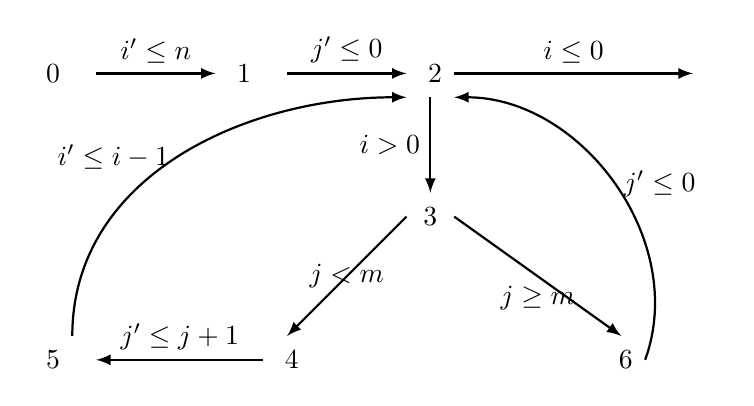
\begin{tikzpicture}[scale=\textwidth/20cm,samples=200]
  \draw[] (-8, 10) circle (0pt) node{{ $0$}};
  \draw[] (-4, 10) circle (0pt) node{{ $1$}};
  \draw[] (0, 10) circle (0pt) node{{ $2$}};
  \draw[] (0, 7) circle (0pt) node{{$3$}};
  \draw[] (-3, 4) circle (0pt) node{{ $4$}};
  \draw[] (-8, 4) circle (0pt) node{{ $5$}};
  \draw[] (4, 4) circle (0pt) node{{ $6$}};
  % Counter Variables
  \draw[] (6, 10) circle (0pt) node {\textbf{$\lex$}};
  %
  % Control Flow Edges:
  \draw[ thick, -latex] (-7, 10)  -- node [above] {$i' \leq n$}(-4.5, 10);
  \draw[ thick, -latex] (-3, 10)  -- node [above] {$j' \leq 0$}(-0.5, 10);
  \draw[ thick, -latex] (0, 9.5)  -- node [left] {$i > 0$} (0, 7.5) ;
  \draw[ thick, -latex] (0.5, 7)  -- node [below] {$ j \geq m $}  (4, 4.5);
  \draw[ thick, -latex] (-7.5, 4.5)  to  [out=90,in=180]  node [left] {$i' \leq i - 1$ }(-0.5, 9.5);
  \draw[ thick, -latex] (4.5, 4)  to  [out=70,in=0]   node [right] {$j' \leq 0 $}(0.5, 9.5);
  \draw[ thick, -latex]  (-0.5, 7) -- node  {$j < m$}  (-3, 4.5) ;
  \draw[ thick, -latex]  (-3.5, 4) -- node [above] {$j' \leq j + 1$}  (-7, 4) ;
  \draw[ thick, -latex] (0.5, 10)  -- node [above] {$i \leq 0$}  (5.5, 10);
  \end{tikzpicture}
  \caption{}
    \end{centering}
    \end{subfigure}
  \caption{
  (a) A simple loop example with two loop paths.
    (b) The corresponding abstract transition graph.}
      \label{fig:twoPathsWhile_abscfg}
  \end{figure}
  }
The program in Figure~\ref{fig:twoPathsWhile_abscfg}(a) is an example of two paths loop with different reachability-bounds on the control
locations in different paths.
Its abstract control flow graph is shown in Figure~\ref{fig:twoPathsWhile_abscfg}(b).
The edge $(0 \xrightarrow{i' \leq n} 1)$ on the top tells us the command 
$\clabel{\assign{i}{n}}^0$ is executed with a continuation point $1$, and the
command $\clabel{\assign{j}{0}}^1$ will be executed next.
The annotation $i' \leq 0$ is a difference constraint 
computed by $\absexpr$ over
the expression $n$ in the assignment command $\assign{i}{n}$.
It represents that the value of $i$ is less than or equal to value of $n$ after the
execution of $\clabel{\assign{i}{n}}^0$ and before executing $\clabel{\assign{j}{0}}^1$.
Another example constraint $i' \leq i - 1$ on the edge $5 \xrightarrow{i' \leq i - 1} 2$
describes the execution of
 the command at line $5$, 
$\clabel{\assign{i}{i - 1}}^{5}$. 
The $i'$ on the left side of $i' \leq i - 1$ represents the value of $i$ after the assignment operation,
and the right-hand side $i$ stores the value before the assignment.
The boolean constraint $i \leq 0 $ on the edge $2 \xrightarrow{i \leq 0} \lex$, 
represents the negation of the testing guard $\clabel{i > 0}^2$
in the $\ewhile$ command.
$2 \xrightarrow{i \leq 0} \lex$ denotes that $i \leq 0$ must hold in order to perform this transition from program point $2$ to
the program exit. 
\end{example}